\documentclass[]{article}
\usepackage[a4paper, total={15cm,23cm}]{geometry}
\usepackage{fancyhdr}
\usepackage{graphicx}
\usepackage{amsmath}
\usepackage{amssymb}
\usepackage{xcolor}
\usepackage{cancel}
%opening
\title{PH 222 Activity 4}
\author{Benjamin Bauml}
\date{Winter 2021}
\pagestyle{fancy}
\rhead{PH 222}
\chead{Winter 2021}
\lhead{Activity 4}

%Custom Quotation Command
\newcommand{\excerpt}[1]{\colorbox{lightgray}{\parbox{14.8cm}{#1}} \\}

\newcommand{\ev}[4]{\left[ #1 \right]_{#2 = #3}^{#2 = #4}}

\begin{document}

\maketitle

\begin{center}
These problems are borrowed/adapted from Chapter 12 of the \textit{Student Workbook} for \textit{Physics for Scientists and Engineers}.
\end{center}
\section*{Activity 1}%27
\excerpt{
A solid cylinder and a cylindrical shell have the same mass,
same radius, and turn on frictionless, horizontal axles. (The
cylindrical shell has light-weight spokes connecting the shell
to the axle.) A rope is wrapped around each cylinder and
tied to a block. The blocks have the same mass and are held
the same height above the ground. Both blocks are released
simultaneously. The ropes do not slip.
Which block hits the ground first? Or is it a tie? Explain.
}
\begin{center}
	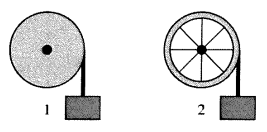
\includegraphics[scale=0.5]{Cylinders}
\end{center}
% To reveal the solution, delete "\phantom{\parbox{\textwidth}{" from the beginning, and "}}" from the end.
\phantom{\parbox{\textwidth}{
The block attached to the solid cylinder hits the ground first. The solid cylinder has a smaller moment of inertia (less of its mass is far from the axle), so it has less resistance to angular acceleration ($ \alpha = \frac{\tau_{net}}{I} $).
%Make this line empty to get a paragraph break when solutions are visible.
We can look at this more mathematically. Let $ T_{1} $ be the tension in the rope attached to the solid cylinder, and let $ T_{2} $ be the tension in the rope attached to the shell. Let $ m $ be the mass of each block, $ M $ be the mass of each cylinder, and $ R $ be the radius of each cylinder. The magnitude of the net force on the block in setup 1 is $ F_{net,1} = mg - T_{1} $, while for setup 2 it is $ F_{net,2} = mg - T_{2} $. The magnitude of net torque on the cylinder in setup 1 is $ \tau_{net,1} = T_{1}R $, while for setup 2 it is $ \tau_{net,2} = T_{2}R $. Since $ F_{net} = ma $ and $ \tau_{net} = I\alpha $, we know that
\[
\begin{split}
	a_{1} & = g-\frac{T_{1}}{m}, \\
	a_{2} & = g-\frac{T_{2}}{m}, \\
	\alpha_{1} & = \frac{T_{1}R}{I_{1}}, \\
	\alpha_{2} & = \frac{T_{2}R}{I_{2}}.
\end{split}
\]
For each cylinder, tangential and angular acceleration are related by $ a_{t} = \alpha R $. Furthermore, since the blocks are connected to the cylinders by ropes that do not slip, the tangential acceleration of each cylinder is equal to the downward acceleration of its attached block. As such,
\[
\begin{split}
	a_{1} & = \alpha_{1}R = \frac{T_{1}R^{2}}{I_{1}}, \\
	a_{2} & = \alpha_{2}R = \frac{T_{2}R^{2}}{I_{2}}.
\end{split}
\]
}}
% To reveal the solution, delete "\phantom{\parbox{\textwidth}{" from the beginning, and "}}" from the end.
\phantom{\parbox{\textwidth}{
For the cylindrical shell, $ I_{2} = MR^{2} $, and for the solid cylinder, $ I_{1} = \frac{1}{2}MR^{2} $. It follows that,
\[
\begin{split}
	a_{1} & = \frac{2T_{1}}{M}, \\
	a_{2} & = \frac{T_{2}}{M}.
\end{split}
\]
Substituting this into the acceleration equations for the blocks, we get
\[
\begin{split}
	a_{1} & = g-\frac{M}{2m}a_{1} \implies a_{1} = \frac{g}{1+\frac{M}{2m}}, \\
	a_{2} & = g-\frac{M}{m}a_{2} \implies a_{2} = \frac{g}{1+\frac{M}{m}}.
\end{split}
\]
As we can see, $ a_{1} > a_{2} $, so the first block will fall faster. If we solve instead for tension, we find
\[
\begin{split}
	T_{1} & = \frac{Ma_{1}}{2} = \frac{Mg}{2+\frac{M}{m}}, \\
	T_{2} & = Ma_{2} = \frac{Mg}{1+\frac{M}{m}}.
\end{split}
\]
Interestingly enough, the tension pulling on the solid cylinder (and thus the net torque) is smaller than the tension pulling on the shell. This is necessary, as if the two tensions were equal, the two boxes (which have the same force of gravity upon them) would fall at the same rate.
}}

\section*{Activity 2}%28
\excerpt{
A metal bar of mass M and length L can rotate in a horizontal
plane about a vertical, frictionless axle through its center.
A hollow channel down the bar allows compressed air (fed
in at the axle) to spray out of two small holes at the ends of
the bar, as shown. The bar is found to speed up to angular
velocity $ \omega $ in a time interval $ \Delta t $, starting from rest. What
force does each escaping jet of air exert on the bar?
}
\begin{center}
	\includegraphics[scale=0.5]{AirBar}
	%\includegraphics[scale=0.5]{AirBarSol}%Solution
\end{center}
\excerpt{
a) \underline{On the figure}, draw vectors to show the forces exerted on
the bar. Then label the radial distance from the axle to the point of application of each force.
}
\excerpt{
b) The forces in your drawing exert a torque about the axles.
Write an expression for each torque, and then add them to get
the net torque. Your expression should be in terms of the unknown force $ F $ and ``known'' quantities
such as $ M $, $ L $, $ g $, etc.
}
% To reveal the solution, delete "\phantom{\parbox{\textwidth}{" from the beginning, and "}}" from the end.
\phantom{\parbox{\textwidth}{
Each individual torque has magnitude $ \tau = rF\sin(90^{\circ}) = (L/2)F $. They point in the same direction (encouraging counterclockwise rotation), so they add to $ \tau_{net} = LF $. \\
}}
\excerpt{
c) What is the moment of inertia of this bar about the axle?
}
% To reveal the solution, delete "\phantom{\parbox{\textwidth}{" from the beginning, and "}}" from the end.
\phantom{\parbox{\textwidth}{
The linear density of the rod is $ \lambda = m/L $. We can view this linear density as $ \lambda = \frac{dm}{dr_{\bot}} $, where $ r_{\bot} $ is the radial coordinate along the rod measured from the axle. As such, $ dm = \frac{m}{L}dr_{\bot} $, and
\[
I = \int r_{\bot}^{2} dm = \int_{-L/2}^{L/2} \frac{mr_{\bot}^{2}}{L} dr_{\bot} = \frac{m}{3L} \left[r_{\bot}^{3}\right]^{L/2}_{r_{\bot}=-L/2} = \frac{m}{3L}\left[\left(\frac{L}{2}\right)^{3}-\left(-\frac{L}{2}\right)^{3}\right]= \frac{1}{12}mL^{2}.
\]
}}
\excerpt{
d) According to Newton's second law, the torque causes the bar to undergo an angular acceleration.
Use your results from parts (b) and (c) to write an expression for the angular acceleration. Simplify the
expression as much as possible.
}
% To reveal the solution, delete "\phantom{\parbox{\textwidth}{" from the beginning, and "}}" from the end.
\phantom{\parbox{\textwidth}{
We know that $ \tau_{net} = I\alpha $. Rearranging this, we find
\[
\alpha = \frac{\tau_{net}}{I} = \frac{LF}{\frac{1}{12}mL^{2}} = \frac{12F}{mL}
\]
}}
\excerpt{
e) You can now use rotational kinematics to write an expression for the bar's angular velocity after time
$ \Delta t $ has elapsed. Do so.
}
% To reveal the solution, delete "\phantom{\parbox{\textwidth}{" from the beginning, and "}}" from the end.
\phantom{\parbox{\textwidth}{
\[
\omega = \omega_{0} + \alpha \Delta t = \alpha\Delta t = \frac{12F}{mL}\Delta t
\]
}}
\excerpt{
f) Finally, solve your equation in part (e) for the unknown force.
}
% To reveal the solution, delete "\phantom{\parbox{\textwidth}{" from the beginning, and "}}" from the end.
\phantom{\parbox{\textwidth}{
\[
F = \frac{mL\omega}{12\Delta t}
\]
}}

\section*{Activity 3}%31
\excerpt{
Forces $ \vec{F}_{1} $ and $ \vec{F}_{2} $
to the comers of a square plate. Is there a single force $ \vec{F}_{3} $ that,
if applied to the appropriate point on the plate, will cause the
plate to be in total equilibrium? If so, draw it, making sure it
has the right position, orientation, and length. If not, explain
why not.
}
\begin{center}
	\includegraphics[scale=0.5]{SquarePlate}
	%\includegraphics[scale=0.5]{SquarePlateSol}%Solution
\end{center}
% To reveal the solution, delete "\phantom{\parbox{\textwidth}{" from the beginning, and "}}" from the end.
\phantom{\parbox{\textwidth}{
Since $ \vec{F}_{1} + \vec{F}_{2} $ is the current net force on the plate, we know that $ \vec{F}_{3} = -(\vec{F}_{1} + \vec{F}_{2}) $ to keep the plate in translational equilibrium with zero net force. What remains is to find if we can position the force to counteract the current net torque.
%Make this line empty to get a paragraph break when solutions are visible.
If we let $ a $ be the side length of the plate, then both $ \vec{F}_{1} $ and $ \vec{F}_{2} $ are applied at a distance $ a/\sqrt{2} $ from the center of mass, with an angle of $ 45^{\circ} $ between the position and force vectors in each case. The forces are both trying to turn the plate counterclockwise, so the torques add together:
\[
\tau_{1} + \tau_{2} = \frac{a}{\sqrt{2}}F\sin(45^{\circ}) + \frac{a}{\sqrt{2}}F\sin(45^{\circ}) = \frac{a}{2}F + \frac{a}{2}F = aF.
\]
}}
% To reveal the solution, delete "\phantom{\parbox{\textwidth}{" from the beginning, and "}}" from the end.
\phantom{\parbox{\textwidth}{
We need $ \tau_{3} = aF $ in the opposite direction. Let $ F = F_{1} = F_{2} $, therefore $ F_{3} = \sqrt{2}F $. Applied to the upper left corner of the plate, $ \vec{F}_{3} $ is applied at a distance $ a/\sqrt{2} $ from the center of mass, with an angle of $ 90^{\circ} $ between the position and force vectors. That means $ \tau_{3} = \frac{a}{\sqrt{2}}(\sqrt{2}F) = aF $, as we desire, and the force acts to turn the plate clockwise, opposing the other two.
}}

\section*{Activity 4}%38
\excerpt{
Rank in order, from largest to smallest, the angular momenta $ L_{1} $ to $ L_{4} $.
}
\begin{center}
	\includegraphics[scale=0.5]{PointMomenta}
\end{center}
% To reveal the solution, delete "\phantom{\parbox{\textwidth}{" from the beginning, and "}}" from the end.
\phantom{\parbox{\textwidth}{
Order: $ L_{3} > L_{4} > L_{2} = L_{1} $ \\
Explanation: $ L = |\vec{r}\times\vec{p}| = rp\sin\theta $, and when the position vector for the point of application and the momentum are at right angles, the magnitude is just $ L = rp = rmv $.
\[
\begin{matrix}
	L_{1} = r_{0}m_{0}v_{0}, & L_{2} = \frac{r_{0}}{2}m_{0}(2v_{0}), \\
	L_{3} = 2r_{0}m_{0}v_{0}, & L_{4} = r_{0}(3m_{0})\frac{v_{0}}{2}.
\end{matrix}
\]
}}

\section*{Activity 5}%39
\excerpt{
Disks 1 and 2 have equal mass. Is the angular
momentum of disk 2 larger than, smaller than,
or equal to the angular momentum of disk 1?
Explain.
}
\begin{center}
	\includegraphics[scale=0.5]{TwoDisks}
\end{center}
% To reveal the solution, delete "\phantom{\parbox{\textwidth}{" from the beginning, and "}}" from the end.
\phantom{\parbox{\textwidth}{
As it happens, $ L_{2} > L_{1} $. Let $ m = m_{1} = m_{2} $. We know that $ L = I\omega = \frac{1}{2}mr^{2}\omega $ for a solid disk. As such, $ L_{1} = \frac{1}{2}mr_{1}^{2}\omega_{1} $ and $ L_{2} = \frac{1}{2}m(2r_{1})^{2}(\frac{1}{2}\omega_{1}) = mr_{1}^{2}\omega_{1} = 2L_{1} $.
}}

\end{document}